\section{Results and analysis}

This section presents the empirical evaluation results and comparative analysis of the proposed multimodal recommendation frameworks. We evaluate 24 distinct configurations across three GNN models (BM3, CombiGCN, and FREEDOM) and one collaborative filtering baseline (LightGCN) under varying encoders and modal fusion strategies. The results are structured to systematically address the four research questions (RQs) defined in Section 4.2.

\subsection{Encoder Comparison}

We first evaluate the impact of different visual feature extractors---CLIP versus MobileNetV2 (MBNv2)---on top-$N$ recommendation accuracy. Visual features represent a critical modality in the fashion rental domain, conveying compatibility and aesthetic styling information. To examine how each encoder influences collaborative filtering under different configurations, we analyze performance along two dimensions: metric consistency across $K$ retrieval levels and multi-dimensional balance across all six evaluation metrics.

\subsubsection{Stability and Peak Performance (Line Plot Analysis)}

The top-$N$ metric line plots in Figure~\ref{fig:encoder_line_comparison} display the performance curves of the evaluated configurations across recommendation list sizes $K \in \{1, 5, 10, 20\}$ under the CLIP encoder (Figure~\ref{fig:metrics_clip}) and the MobileNetV2 encoder (Figure~\ref{fig:metrics_mbnv2}). Red stars highlight the optimal configuration for each metric at each $K$ level.

\begin{figure}[H]
    \centering
    \begin{subfigure}[b]{0.48\textwidth}
        \centering
        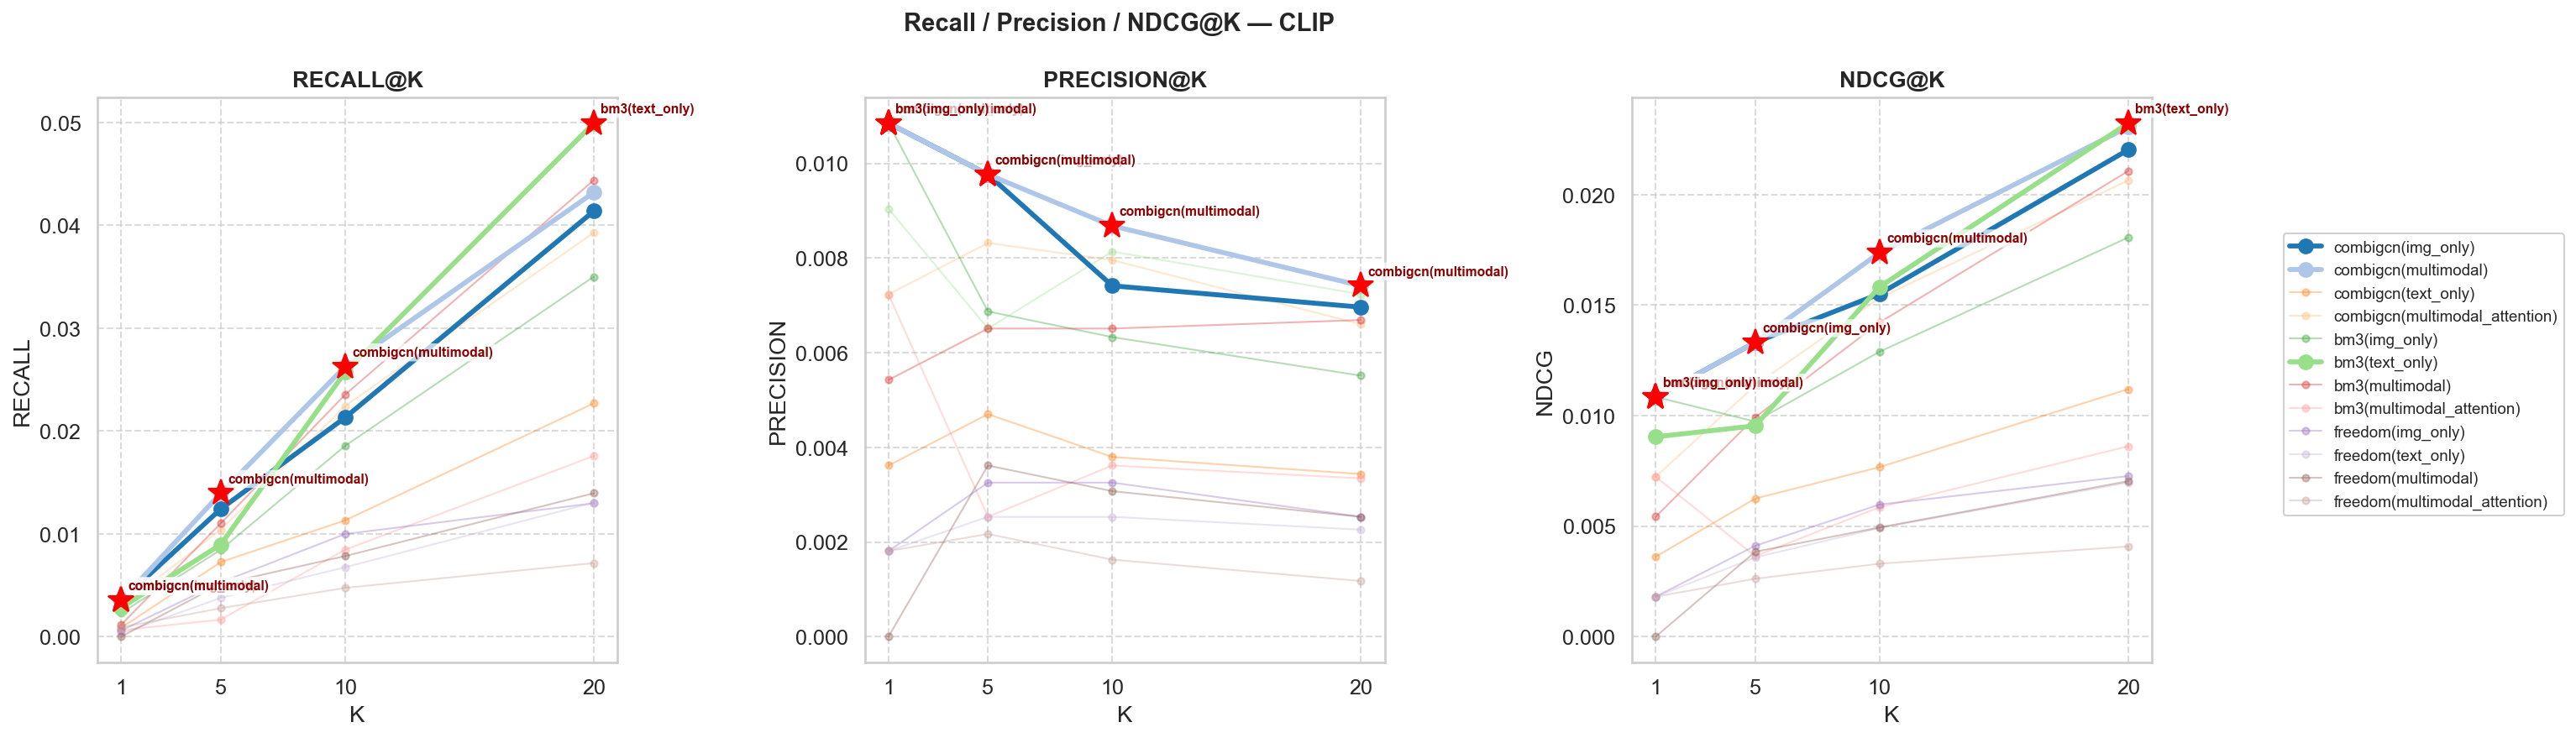
\includegraphics[width=\textwidth]{figs/chap4/Figure_46_Recall_Precision_NDCG_K_CLIP.png}
        \caption{CLIP Encoder Configurations}
        \label{fig:metrics_clip}
    \end{subfigure}
    \hfill
    \begin{subfigure}[b]{0.48\textwidth}
        \centering
        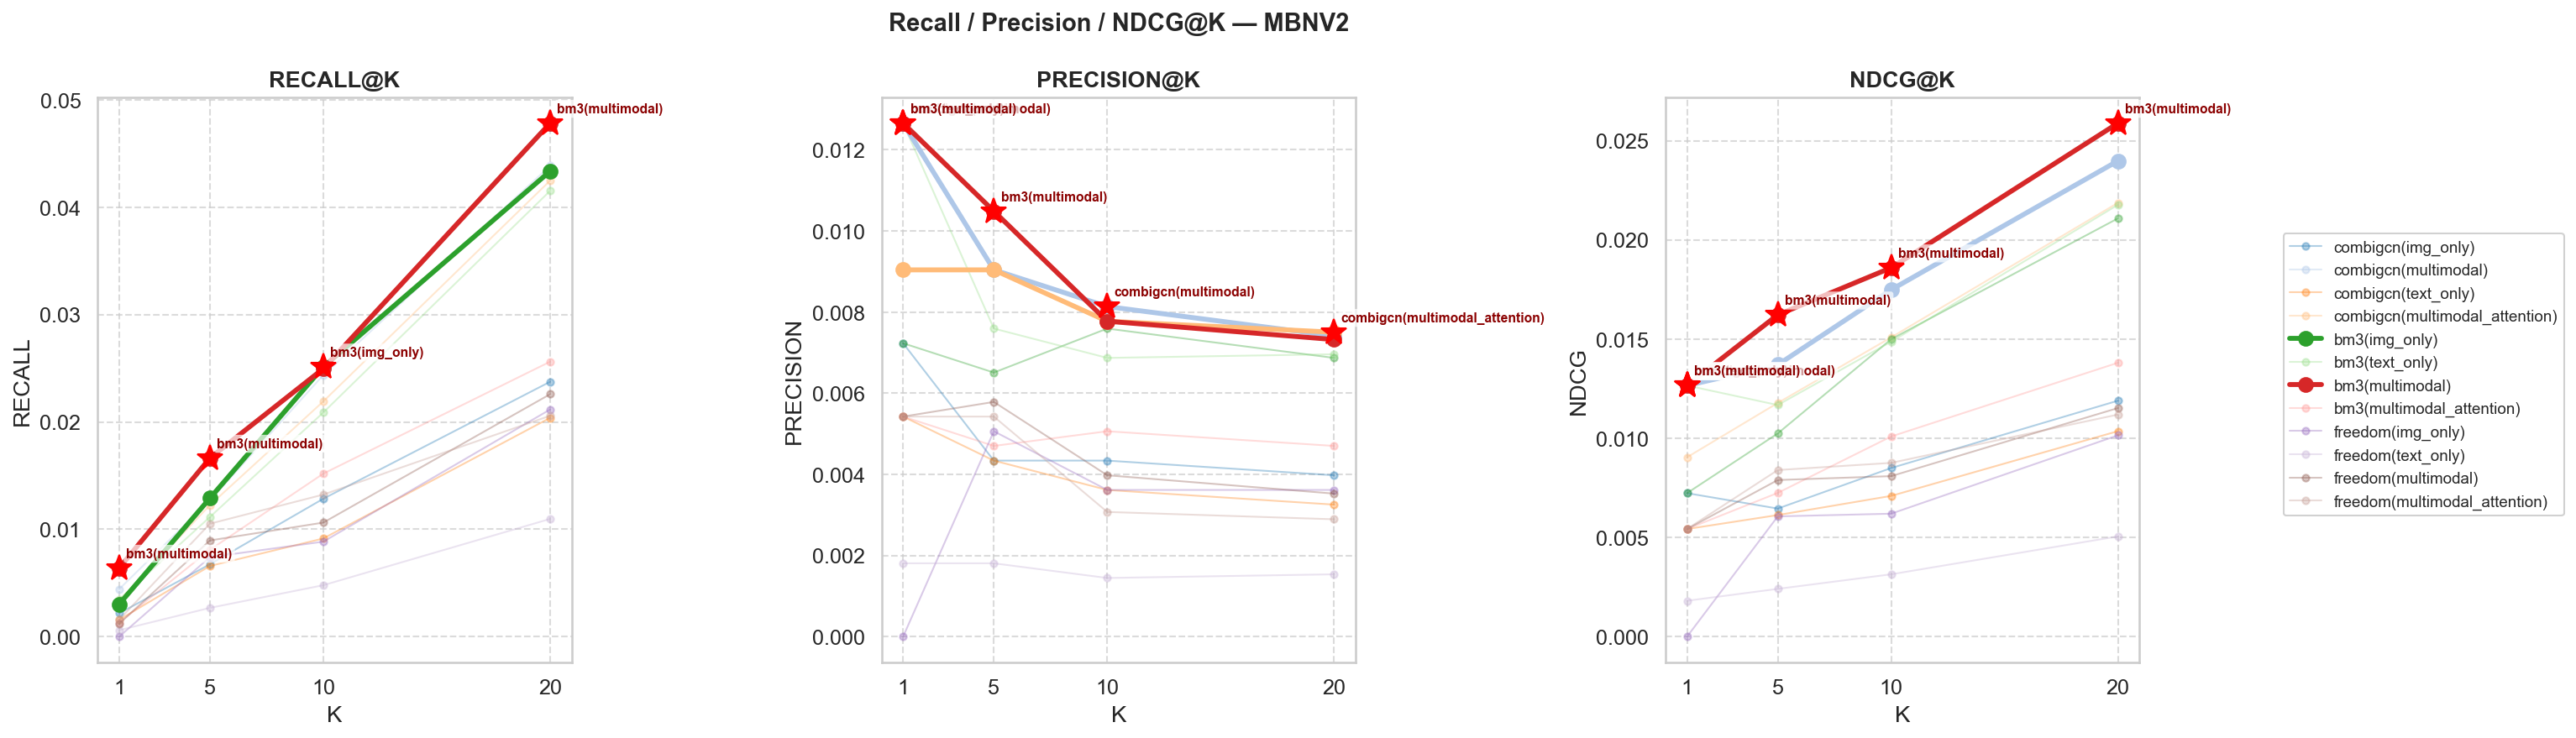
\includegraphics[width=\textwidth]{figs/chap4/Figure_47_Recall_Precision_NDCG_K_MBNV2.png}
        \caption{MobileNetV2 (MBNv2) Encoder Configurations}
        \label{fig:metrics_mbnv2}
    \end{subfigure}
    \caption{Top-$N$ recommendation performance (Recall@K, Precision@K, NDCG@K) of various model configurations under CLIP and MobileNetV2 encoders across different values of $K \in \{1, 5, 10, 20\}$. Red stars highlight the optimal configuration for each metric at each $K$ level.}
    \label{fig:encoder_line_comparison}
\end{figure}

Under the CLIP encoder (Figure~\ref{fig:metrics_clip}), we observe a significant lack of configuration consistency. The best-performing model setup shifts frequently as the ranking size $K$ changes. For instance, on the Recall metric, the hybrid collaborative filtering model CombiGCN under the \texttt{multimodal} late fusion setting leads at lower recall thresholds ($K \in \{1, 5, 10\}$) but is surpassed by the text-only configuration of BM3 using TF-IDF (\texttt{bm3\_tfidf}) at $K=20$. Similarly, for the Precision metric, the optimal configuration shifts from the visual-only BM3 (\texttt{bm3\_img\_only}) at $K=1$ to the late-fusion CombiGCN (\texttt{combigcn\_multimodal}) at higher $K$ values. On the NDCG metric, the top configuration changes dynamically across almost all evaluation points (e.g., \texttt{combigcn\_img\_only} at $K=5$, \texttt{combigcn\_multimodal} at $K=10$, and \texttt{bm3\_tfidf} at $K=20$). This performance volatility suggests that CLIP's joint text-image representations do not establish a stable synergy with the collaborative recommendation models for this specific dataset.

Conversely, the MobileNetV2 encoder (Figure~\ref{fig:metrics_mbnv2}) exhibits robust stability and clear convergence towards a single dominant configuration: \texttt{bm3\_multimodal} (highlighted by the bold red line). For both the Recall and NDCG metrics, \texttt{bm3\_multimodal} consistently maintains the lead across all values of $K$. For example, the NDCG@20 of the MBNv2-based \texttt{bm3\_multimodal} exceeds $0.025$, whereas the best CLIP-based configuration peaks at only approximately $0.023$. On the Precision metric, although \texttt{bm3\_multimodal} faces minor competition from \texttt{combigcn\_multimodal} at $K=10$ and \texttt{combigcn\_multimodal\_attention} at $K=20$, it remains highly competitive and stable, showcasing a consistent learning capability.

\subsubsection{Comprehensive Multi-Metric Analysis (Radar Plot Analysis)}

The radar plots in Figure~\ref{fig:encoder_radar_comparison} provide a multi-dimensional perspective across all six evaluation metrics (Recall, Precision, NDCG, MRR, MAP, and Hit Ratio), highlighting the structural balance of the two encoders.

\begin{figure}[H]
    \centering
    \begin{subfigure}[b]{0.48\textwidth}
        \centering
        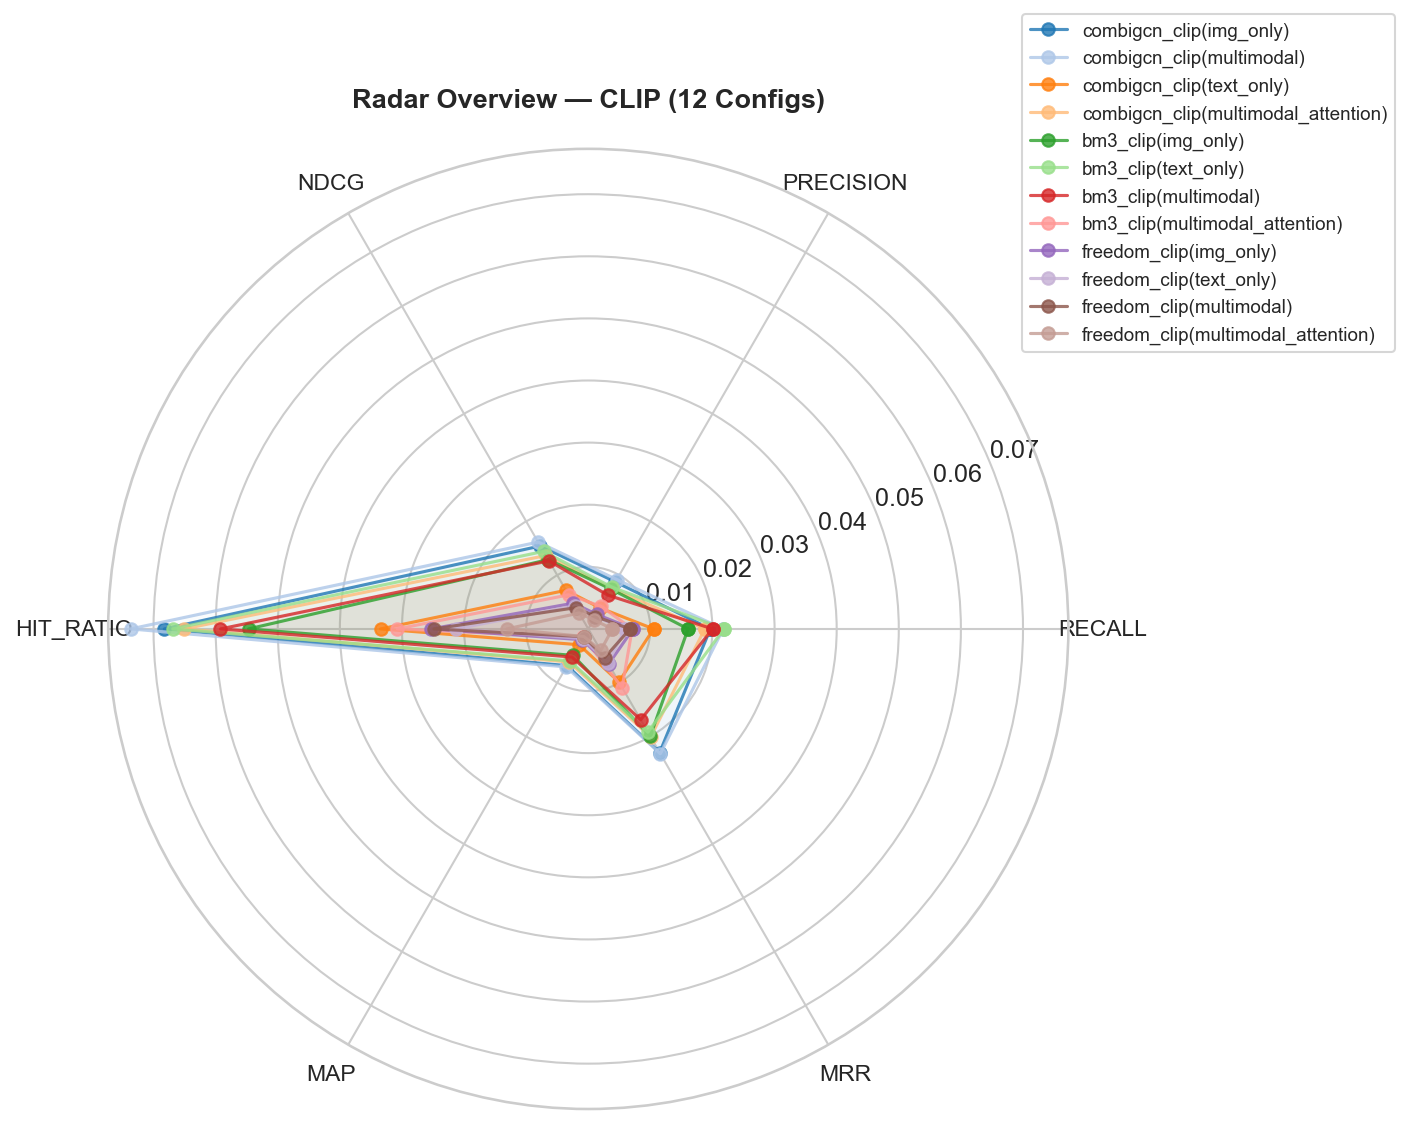
\includegraphics[width=\textwidth]{figs/chap4/Figure_74_Radar_Overview_CLIP_12_Configs.png}
        \caption{CLIP Encoder Configurations}
        \label{fig:radar_clip}
    \end{subfigure}
    \hfill
    \begin{subfigure}[b]{0.48\textwidth}
        \centering
        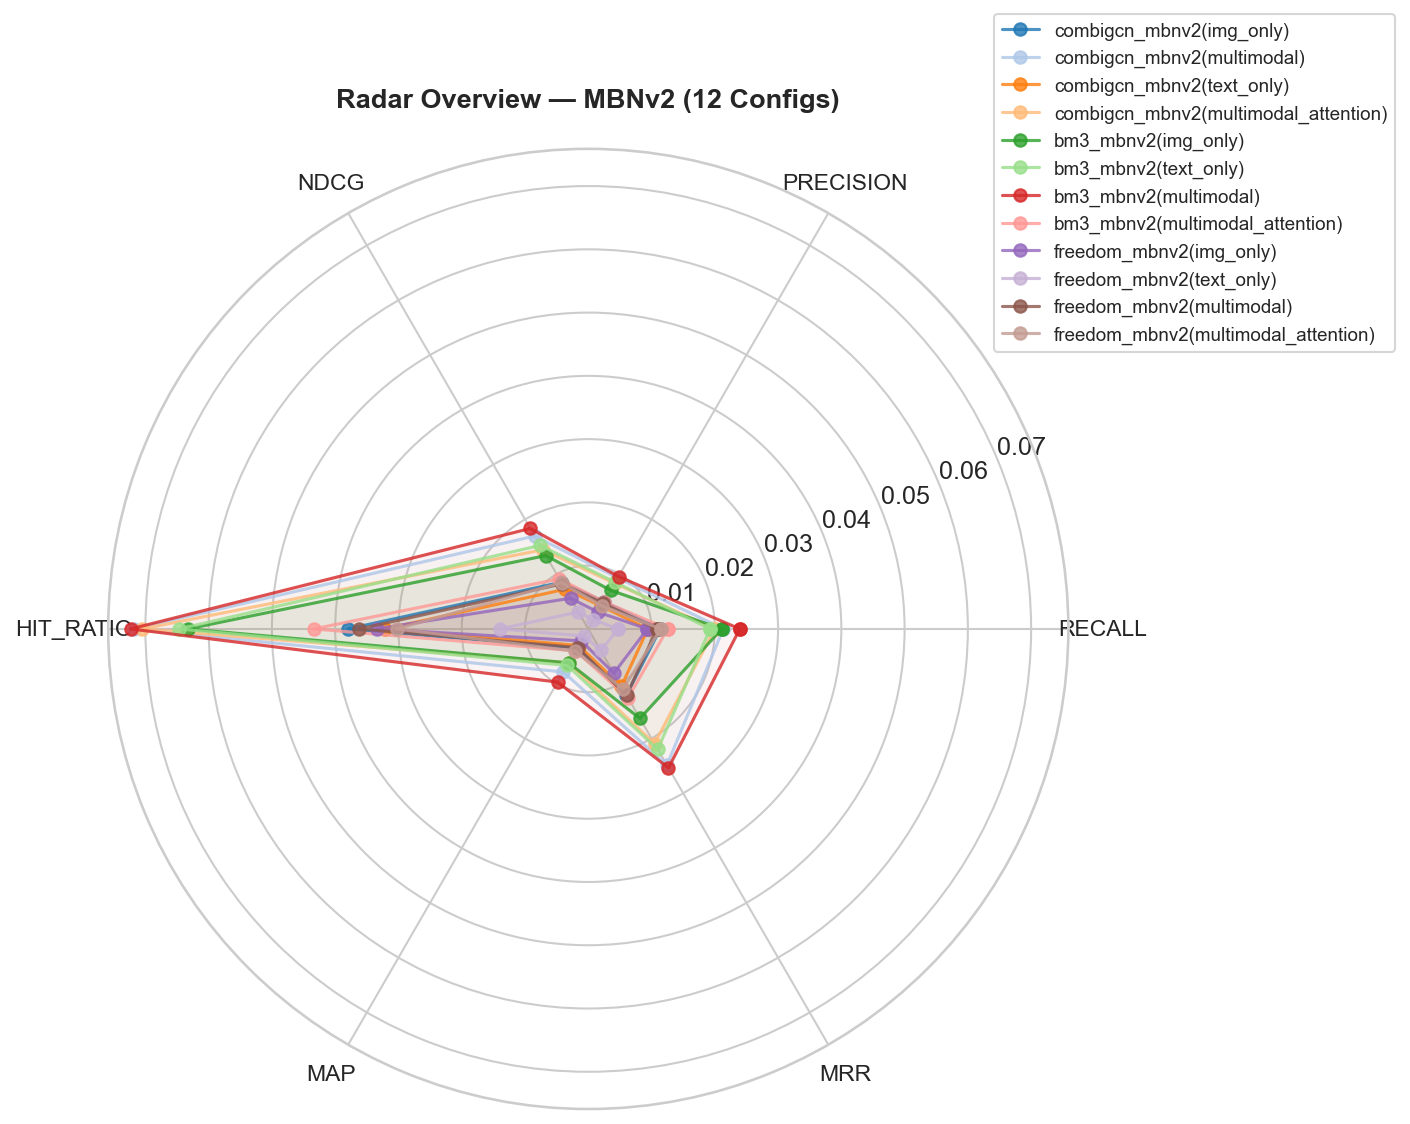
\includegraphics[width=\textwidth]{figs/chap4/Figure_75_Radar_Overview_MBNv2_12_Configs.png}
        \caption{MobileNetV2 (MBNv2) Encoder Configurations}
        \label{fig:radar_mbnv2}
    \end{subfigure}
    \caption{Radar charts summarizing the performance of the evaluated configurations across six recommendation metrics. The MobileNetV2-based \texttt{bm3\_multimodal} configuration exhibits a balanced, widely-expanded polygon compared to the fragmented performance of CLIP-based configurations.}
    \label{fig:encoder_radar_comparison}
\end{figure}

For the CLIP encoder (Figure~\ref{fig:radar_clip}), the performance is highly fragmented. No single configuration dominates across all dimensions, resulting in asymmetrical, collapsed shapes. For instance, while the late-fusion CombiGCN (\texttt{combigcn\_multimodal}) achieves a high Hit Ratio (exceeding $0.07$), its polygon is severely compressed along other metrics. On the other hand, the text-only BM3 (\texttt{bm3\_tfidf}) shows a strong Recall projection (touching $0.05$) but performs poorly on ranking-sensitive metrics such as MAP and MRR. The overall CLIP polygon is heavily compressed in deep ranking metrics (MAP, MRR, and NDCG remaining within the $0.01$--$0.02$ range).

Under the MobileNetV2 encoder (Figure~\ref{fig:radar_mbnv2}), we observe a striking contrast. The polygon representing \texttt{bm3\_multimodal} (red line) is widely expanded and completely encompasses the other configurations. It overcomes the fragmentation issue seen with CLIP by achieving the highest scores not only on the Hit Ratio metric (touching near $0.08$) but also across all core ranking quality metrics, including NDCG, MAP, and MRR.

\subsubsection{Theoretical Discussion and Insights}

The empirical superiority of MobileNetV2 over CLIP in the best-performing configurations highlights an important domain-specific constraint in fashion recommendation. While CLIP is a large, state-of-the-art vision-language foundation model trained on massive image-text pairs, its objective is optimized for high-level, coarse-grained semantic alignment between text descriptions and images. As a result, CLIP's embeddings tend to represent abstract concepts and object classes (e.g., classifying a garment as a ``red dress''). 

However, fashion styling and item compatibility depend on fine-grained visual features, such as local textures, stitching patterns, fabric type, collar shape, and detailed styling lines. MobileNetV2, being a convolutional neural network (CNN) trained with localized spatial pooling, preserves these low-level spatial texture features and local color distributions in its early and middle layers. In collaborative filtering, these fine-grained texture descriptors serve as stronger indicators of aesthetic compatibility than coarse semantic labels. Therefore, when combined with collaborative filtering structures, MobileNetV2 generates more descriptive and stable representations than CLIP, leading to superior and more consistent recommendations.

\subsection{Fusion Strategy Comparison}

We perform an ablation study to analyze the impact of different feature integration strategies---visual-only (\texttt{img\_only}), textual-only (\texttt{tfidf}), multimodal late fusion (\texttt{multimodal}), and weighted attention gating (\texttt{multimodal\_attention})---across the three graph recommendation models.

\subsubsection{Architecture-Specific Ablation Performance}

The ablation performance is analyzed individually for each of the three graphcollaborative filtering models. Figure~\ref{fig:ablation_heatmaps} displays the NDCG@K ablation heatmaps for BM3 (Figure~\ref{fig:ablation_bm3}), CombiGCN (Figure~\ref{fig:ablation_combigcn}), and FREEDOM (Figure~\ref{fig:ablation_freedom}).

\begin{figure}[H]
    \centering
    \begin{subfigure}[b]{0.6\textwidth}
        \centering
        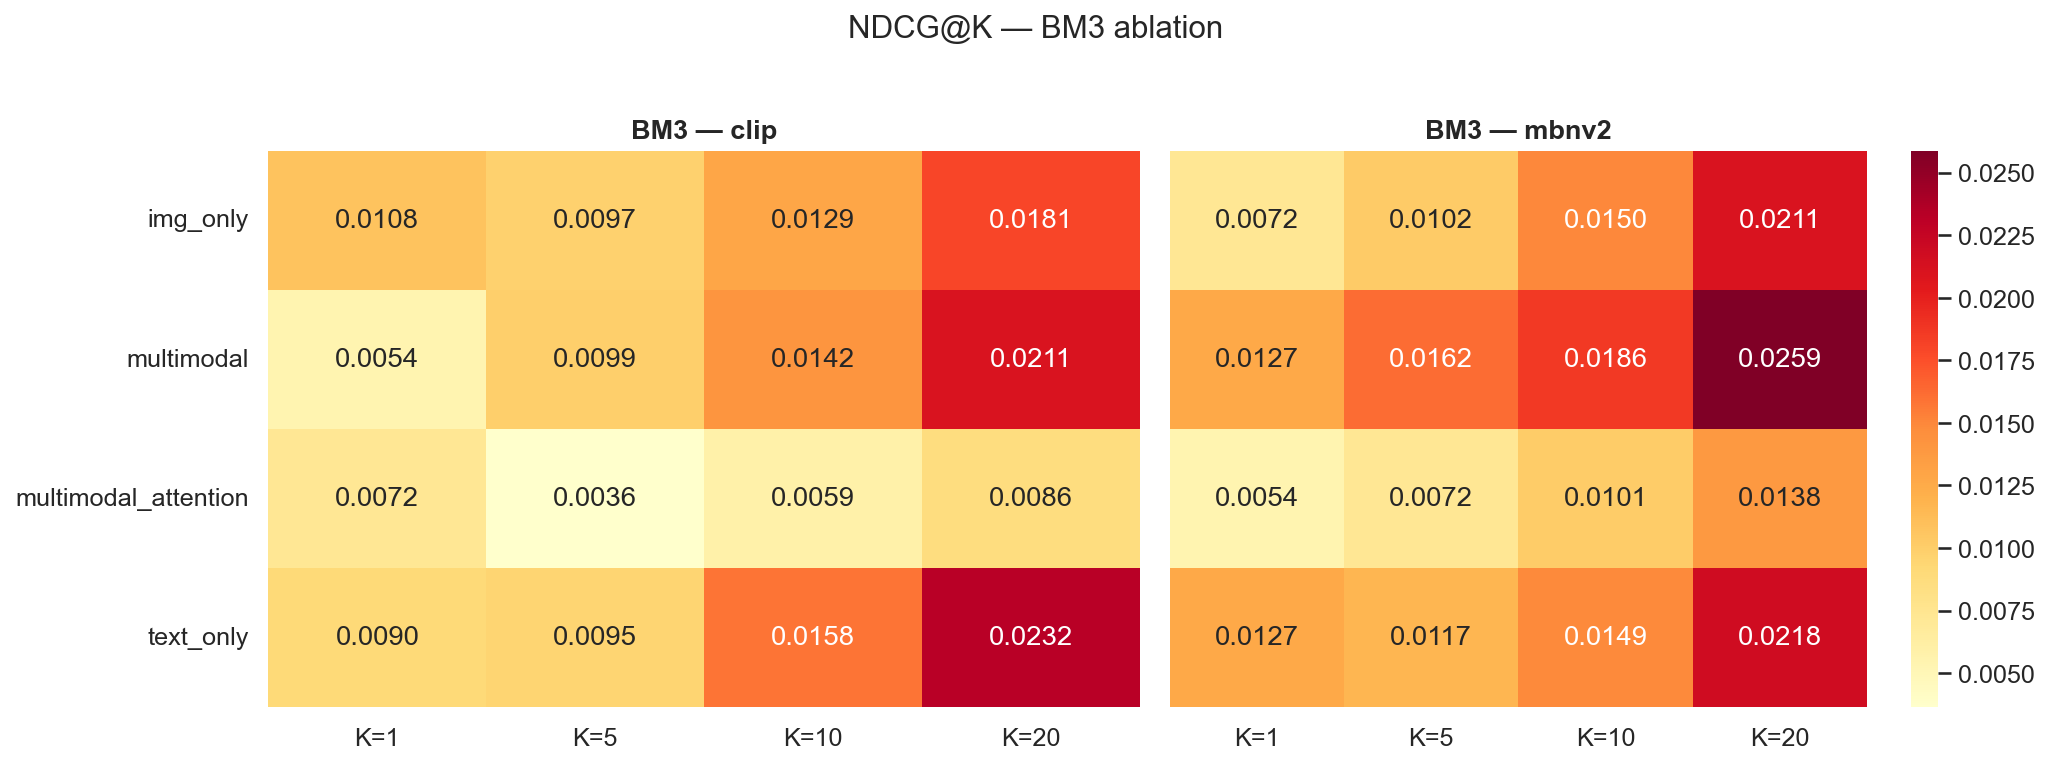
\includegraphics[width=\textwidth]{figs/chap4/Figure_48_NDCG_K_BM3_ablation.png}
        \caption{BM3 Ablation}
        \label{fig:ablation_bm3}
    \end{subfigure}
    
    \vspace{0.4cm}
    \begin{subfigure}[b]{0.6\textwidth}
        \centering
        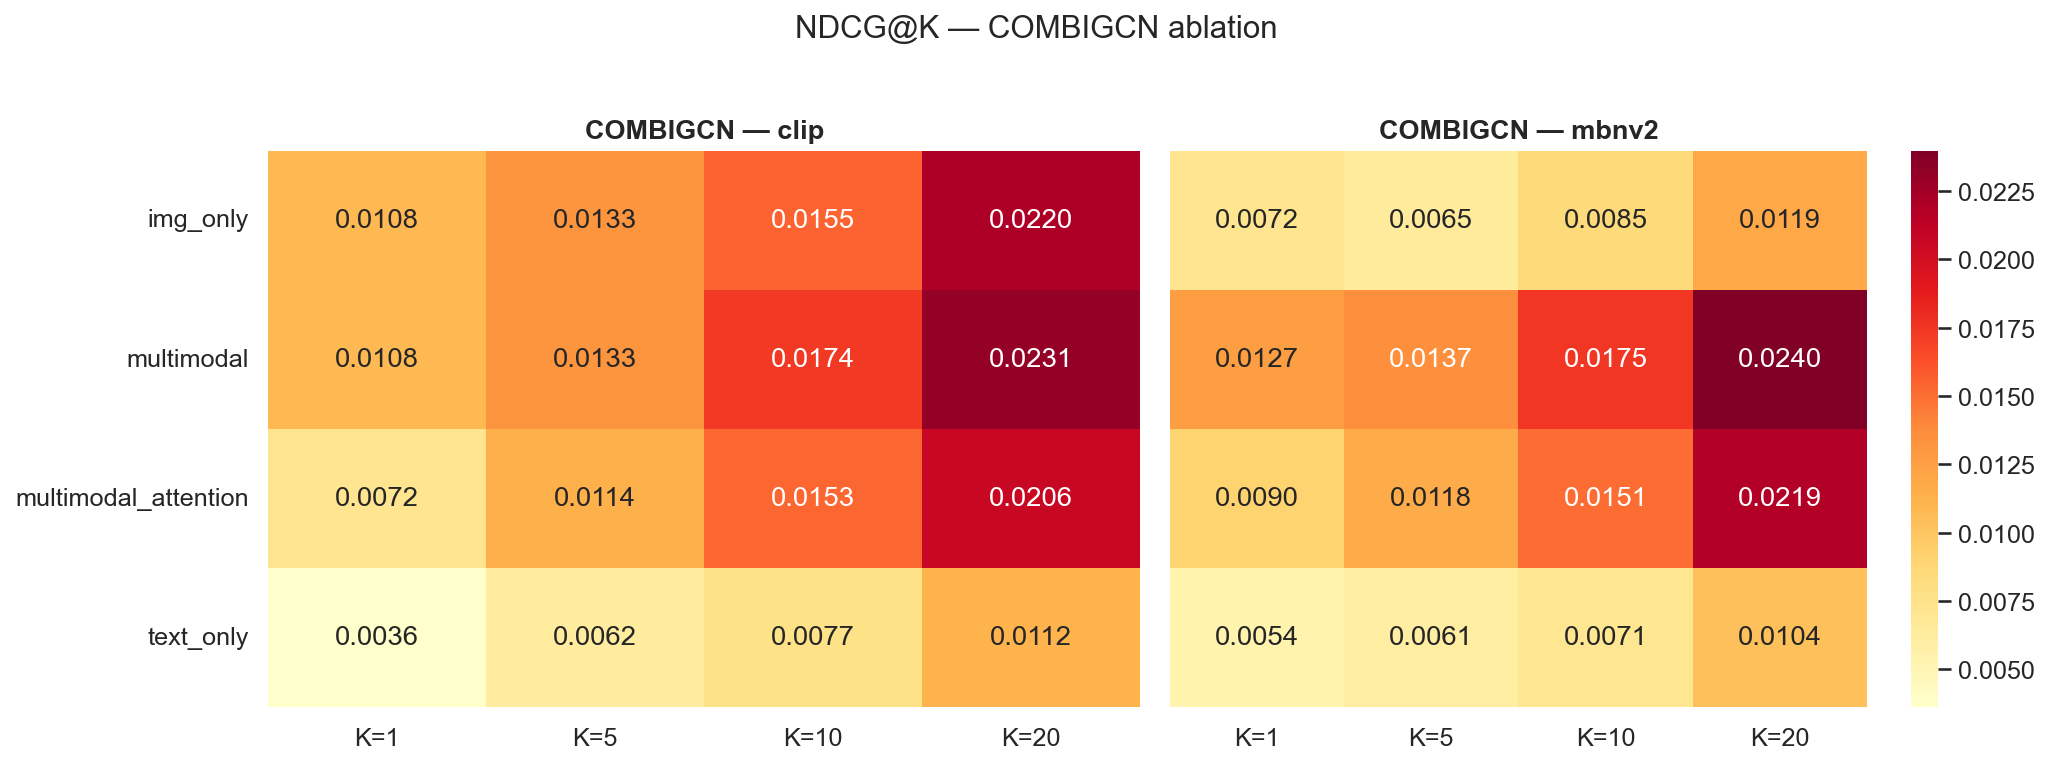
\includegraphics[width=\textwidth]{figs/chap4/Figure_56_NDCG_K_COMBIGCN_ablation.png}
        \caption{CombiGCN Ablation}
        \label{fig:ablation_combigcn}
    \end{subfigure}
    
    \vspace{0.4cm}
    \begin{subfigure}[b]{0.6\textwidth}
        \centering
        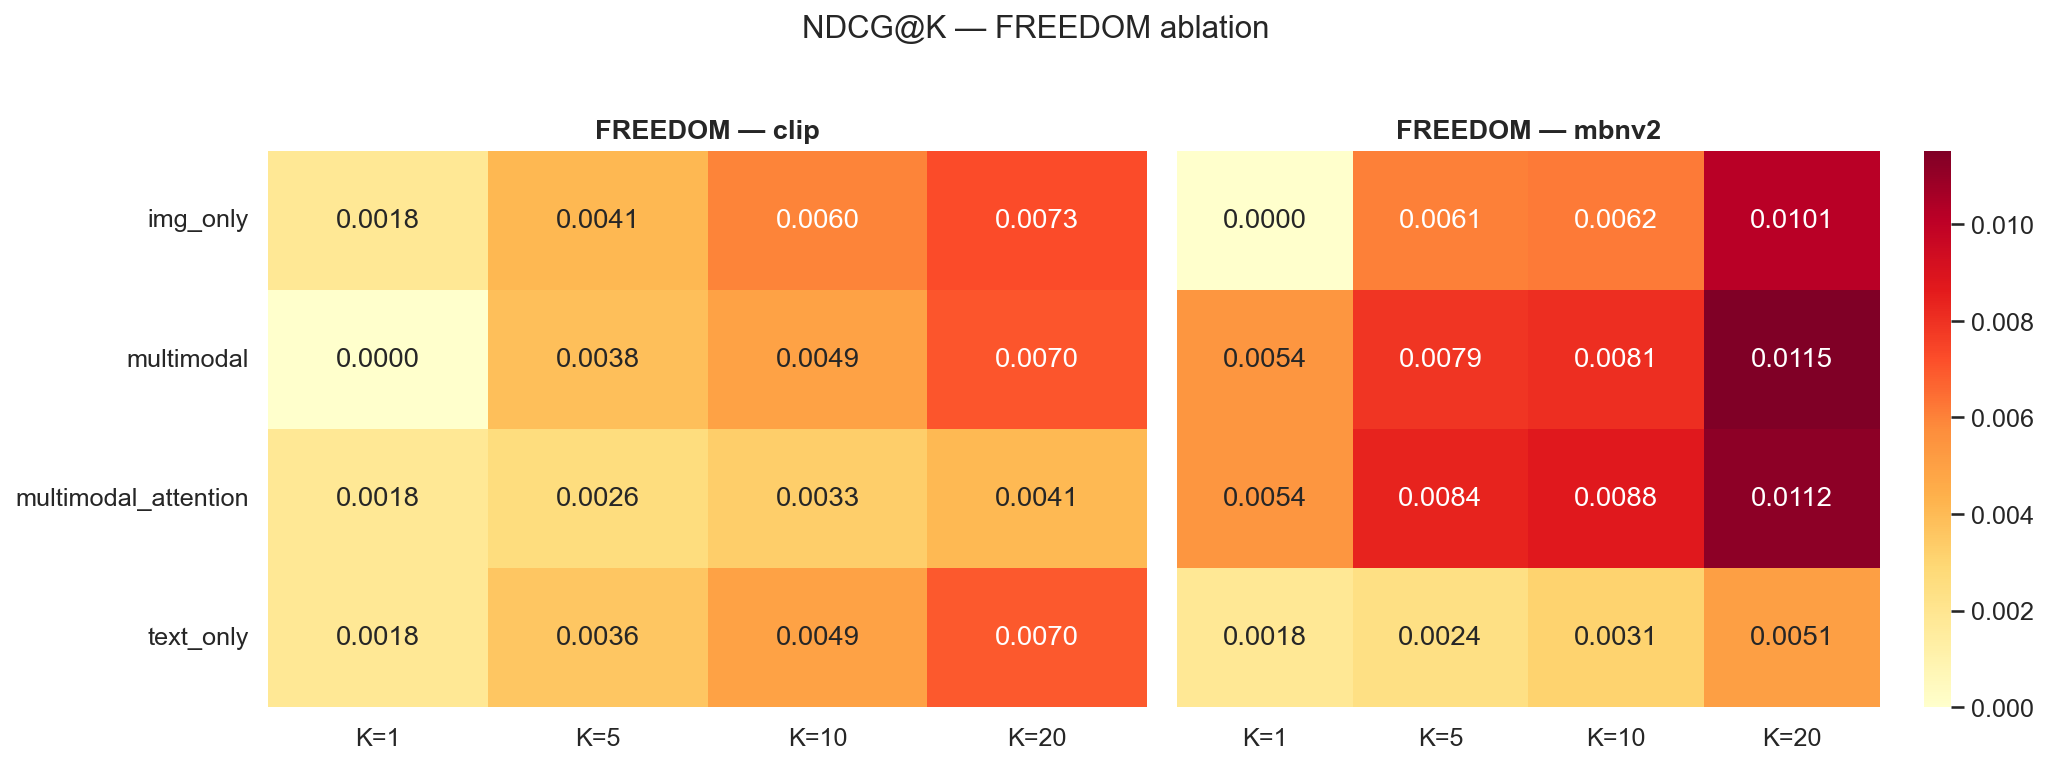
\includegraphics[width=\textwidth]{figs/chap4/Figure_64_NDCG_K_FREEDOM_ablation.png}
        \caption{FREEDOM Ablation}
        \label{fig:ablation_freedom}
    \end{subfigure}
    \caption{NDCG@K ablation heatmaps for BM3, CombiGCN, and FREEDOM architectures across various visual encoders and similarity/fusion types.}
    \label{fig:ablation_heatmaps}
\end{figure}

\paragraph{BM3 Architecture}
As shown in the NDCG@K heatmap (Figure~\ref{fig:ablation_bm3}) and the NDCG@10 comparison (Figure~\ref{fig:bm3_sim_comparison}), the late-fusion \texttt{multimodal} strategy combined with the MBNv2 visual encoder achieves the highest performance. At $K=20$, this configuration reaches an NDCG of $0.0259$ (marked as the darkest red cell), leading all other configurations. An interesting anomaly occurs in the CLIP-based configurations: the traditional textual features (\texttt{tfidf}) outperform the late-fusion \texttt{multimodal} strategy at $K=10$ (NDCG of $0.0158$ for \texttt{tfidf} versus $0.0142$ for \texttt{multimodal}). However, when switching to the MBNv2 encoder, the late fusion strategy resumes its dominant position.

\begin{figure}[H]
    \centering
    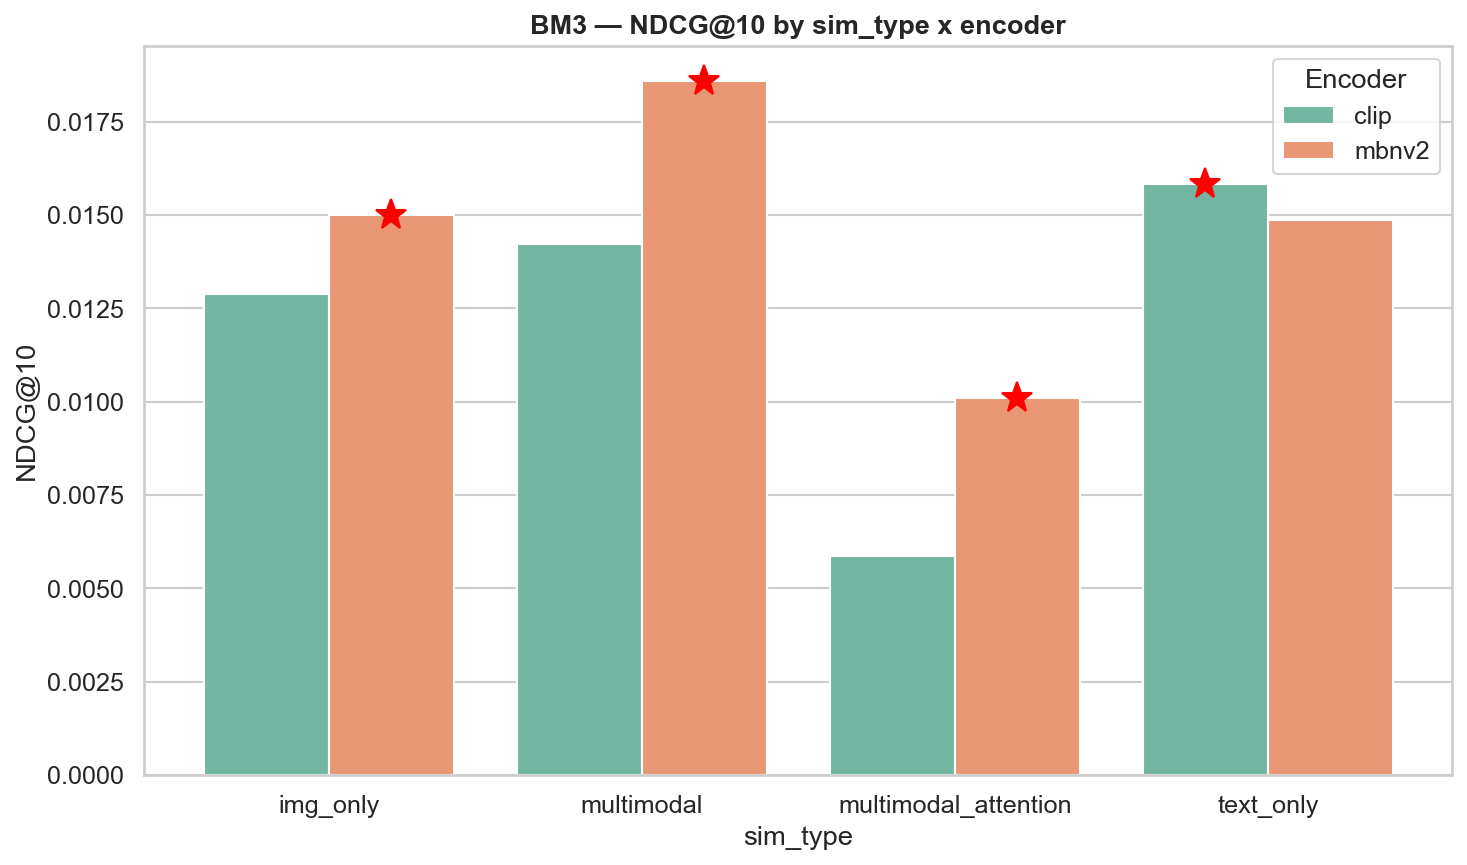
\includegraphics[width=0.7\textwidth]{figs/chap4/Figure_55_BM3_NDCG_10_by_sim_type_x_encoder.png}
    \caption{BM3 performance comparison at NDCG@10 across different similarity/fusion types and visual encoders.}
    \label{fig:bm3_sim_comparison}
\end{figure}

Crucially, the trainable weighted attention gating strategy (\texttt{multimodal\_attention}) fails to improve BM3's performance, causing a severe drop in recommendation quality. As illustrated in Figure~\ref{fig:bm3_sim_comparison}, the NDCG@10 score drops from $0.0186$ (\texttt{multimodal}) to $0.0101$ (\texttt{multimodal\_attention}) under the MBNv2 encoder, representing a $46\%$ degradation. A similar drop of $59\%$ is observed under the CLIP encoder.

\paragraph{CombiGCN Architecture}
As shown in Figure~\ref{fig:ablation_combigcn}, CombiGCN exhibits highly consistent performance under the late-fusion \texttt{multimodal} strategy. Both CLIP and MBNv2 visual encoders achieve their peak performance under this setting (with the MBNv2-based multimodal setting peaking at an NDCG of $0.0240$ at $K=20$). 

However, we observe a notable paradox in the visual-only (\texttt{img\_only}) setting. When only visual embeddings are utilized, the CLIP encoder significantly outperforms MBNv2. For example, at $K=20$, CLIP \texttt{img\_only} achieves an NDCG@20 of $0.0220$, whereas MBNv2 \texttt{img\_only} drops to $0.0119$. Additionally, CombiGCN shows a high level of incompatibility with textual-only features (\texttt{tfidf}). The NDCG scores for CombiGCN \texttt{tfidf} configurations collapse to the bottom of the scale, as shown by the pale yellow band at the bottom of the heatmap in Figure~\ref{fig:ablation_combigcn}.

\paragraph{FREEDOM Architecture}
The overall NDCG values for FREEDOM (Figure~\ref{fig:ablation_freedom}) are significantly lower than those of BM3 and CombiGCN, peaking at only $0.0115$ at $K=20$. Under this architecture, the MBNv2 encoder shows a much stronger performance than CLIP when handling complex settings. For instance, at $K=20$, MBNv2 achieves an NDCG of $0.0115$ and $0.0112$ for \texttt{multimodal} and \texttt{multimodal\_attention} respectively, whereas CLIP drops to $0.0070$ and $0.0041$. The CLIP encoder only outperforms MBNv2 in the textual-only (\texttt{tfidf}) configuration, though the absolute performance remains very low.

\subsubsection{Ablation Synthesis and Discussion}

We summarize the NDCG@10 results in Table~\ref{tab:ablation_summary}, reporting the best encoder performance for each setting.

\begin{table}[H]
\centering
\caption{Ablation Study Comparison of NDCG@10 Scores Under Different Similarity and Fusion Types (Best Encoder Selected for Each Setup).}
\label{tab:ablation_summary}
\small
\setlength{\tabcolsep}{6pt}
\begin{tabular}{lcccc}
\hline
\textbf{Model} & \textbf{img\_only} & \textbf{tfidf} & \textbf{multimodal} & \shortstack[c]{\textbf{multimodal\_}\\\textbf{attention}} \\ \hline
BM3 (MBNv2) & 0.0150 & 0.0149 & \textbf{0.0186} & 0.0101 \\
CombiGCN (MBNv2) & 0.0085 & 0.0071 & \textbf{0.0175} & 0.0151 \\
FREEDOM (MBNv2) & 0.0062 & 0.0031 & 0.0081 & \textbf{0.0088} \\ \hline
\end{tabular}
\end{table}

From the ablation experiments, we derive three key insights:
\begin{enumerate}
    \item \textbf{Late Fusion (\texttt{multimodal}) is the optimal strategy}: For robust GNN models (BM3 and CombiGCN), combining visual and textual features via late fusion outperforms single-modality setups. The poor performance of textual-only (\texttt{tfidf}) configurations confirms that visual features represent the dominant modality in fashion recommendation, as consumers prioritize visual aesthetics and styling compatibility.
    \item \textbf{Weighted attention gating (\texttt{multimodal\_attention}) is not a universal improvement}: Attention gating degrades BM3 by $46\%$ and CombiGCN by $14\%$. It only improves FREEDOM by $+8\%$. This indicates that for models with strong modal representation learning (such as contrastive alignment in BM3 or dual-graph propagation in CombiGCN), adding a trainable attention gating layer increases model complexity and introduces overfitting and noise on this smaller dataset (9,455 interactions). FREEDOM is weaker overall, so the attention gating provides a small regularization/guidance benefit, but it remains far below the other architectures.
    \item \textbf{No universal configuration (no silver bullet)}: Configuration choices are highly architecture-dependent. BM3 is highly compatible with TF-IDF under CLIP, whereas CombiGCN is incompatible with TF-IDF but achieves high performance with CLIP-based visual-only embeddings. Therefore, encoder and fusion settings must be optimized locally for each specific recommender structure.
\end{enumerate}

\subsection{Model Comparison}

We compare the best-performing configuration of each architecture to identify the most effective overall recommendation framework for the VCR dataset. Both BM3 and CombiGCN achieve their best performance under the MBNv2-based multimodal late fusion setting, whereas FREEDOM peaks under the MBNv2-based weighted attention fusion setting. This reinforces the findings in RQ1 regarding the superiority of MobileNetV2.

\subsubsection{Performance Trade-Offs (Bar Chart Analysis)}

The best configurations of BM3, CombiGCN, and FREEDOM are compared across all six evaluation metrics in Figure~\ref{fig:best_config_overview}.

\begin{figure}[H]
    \centering
    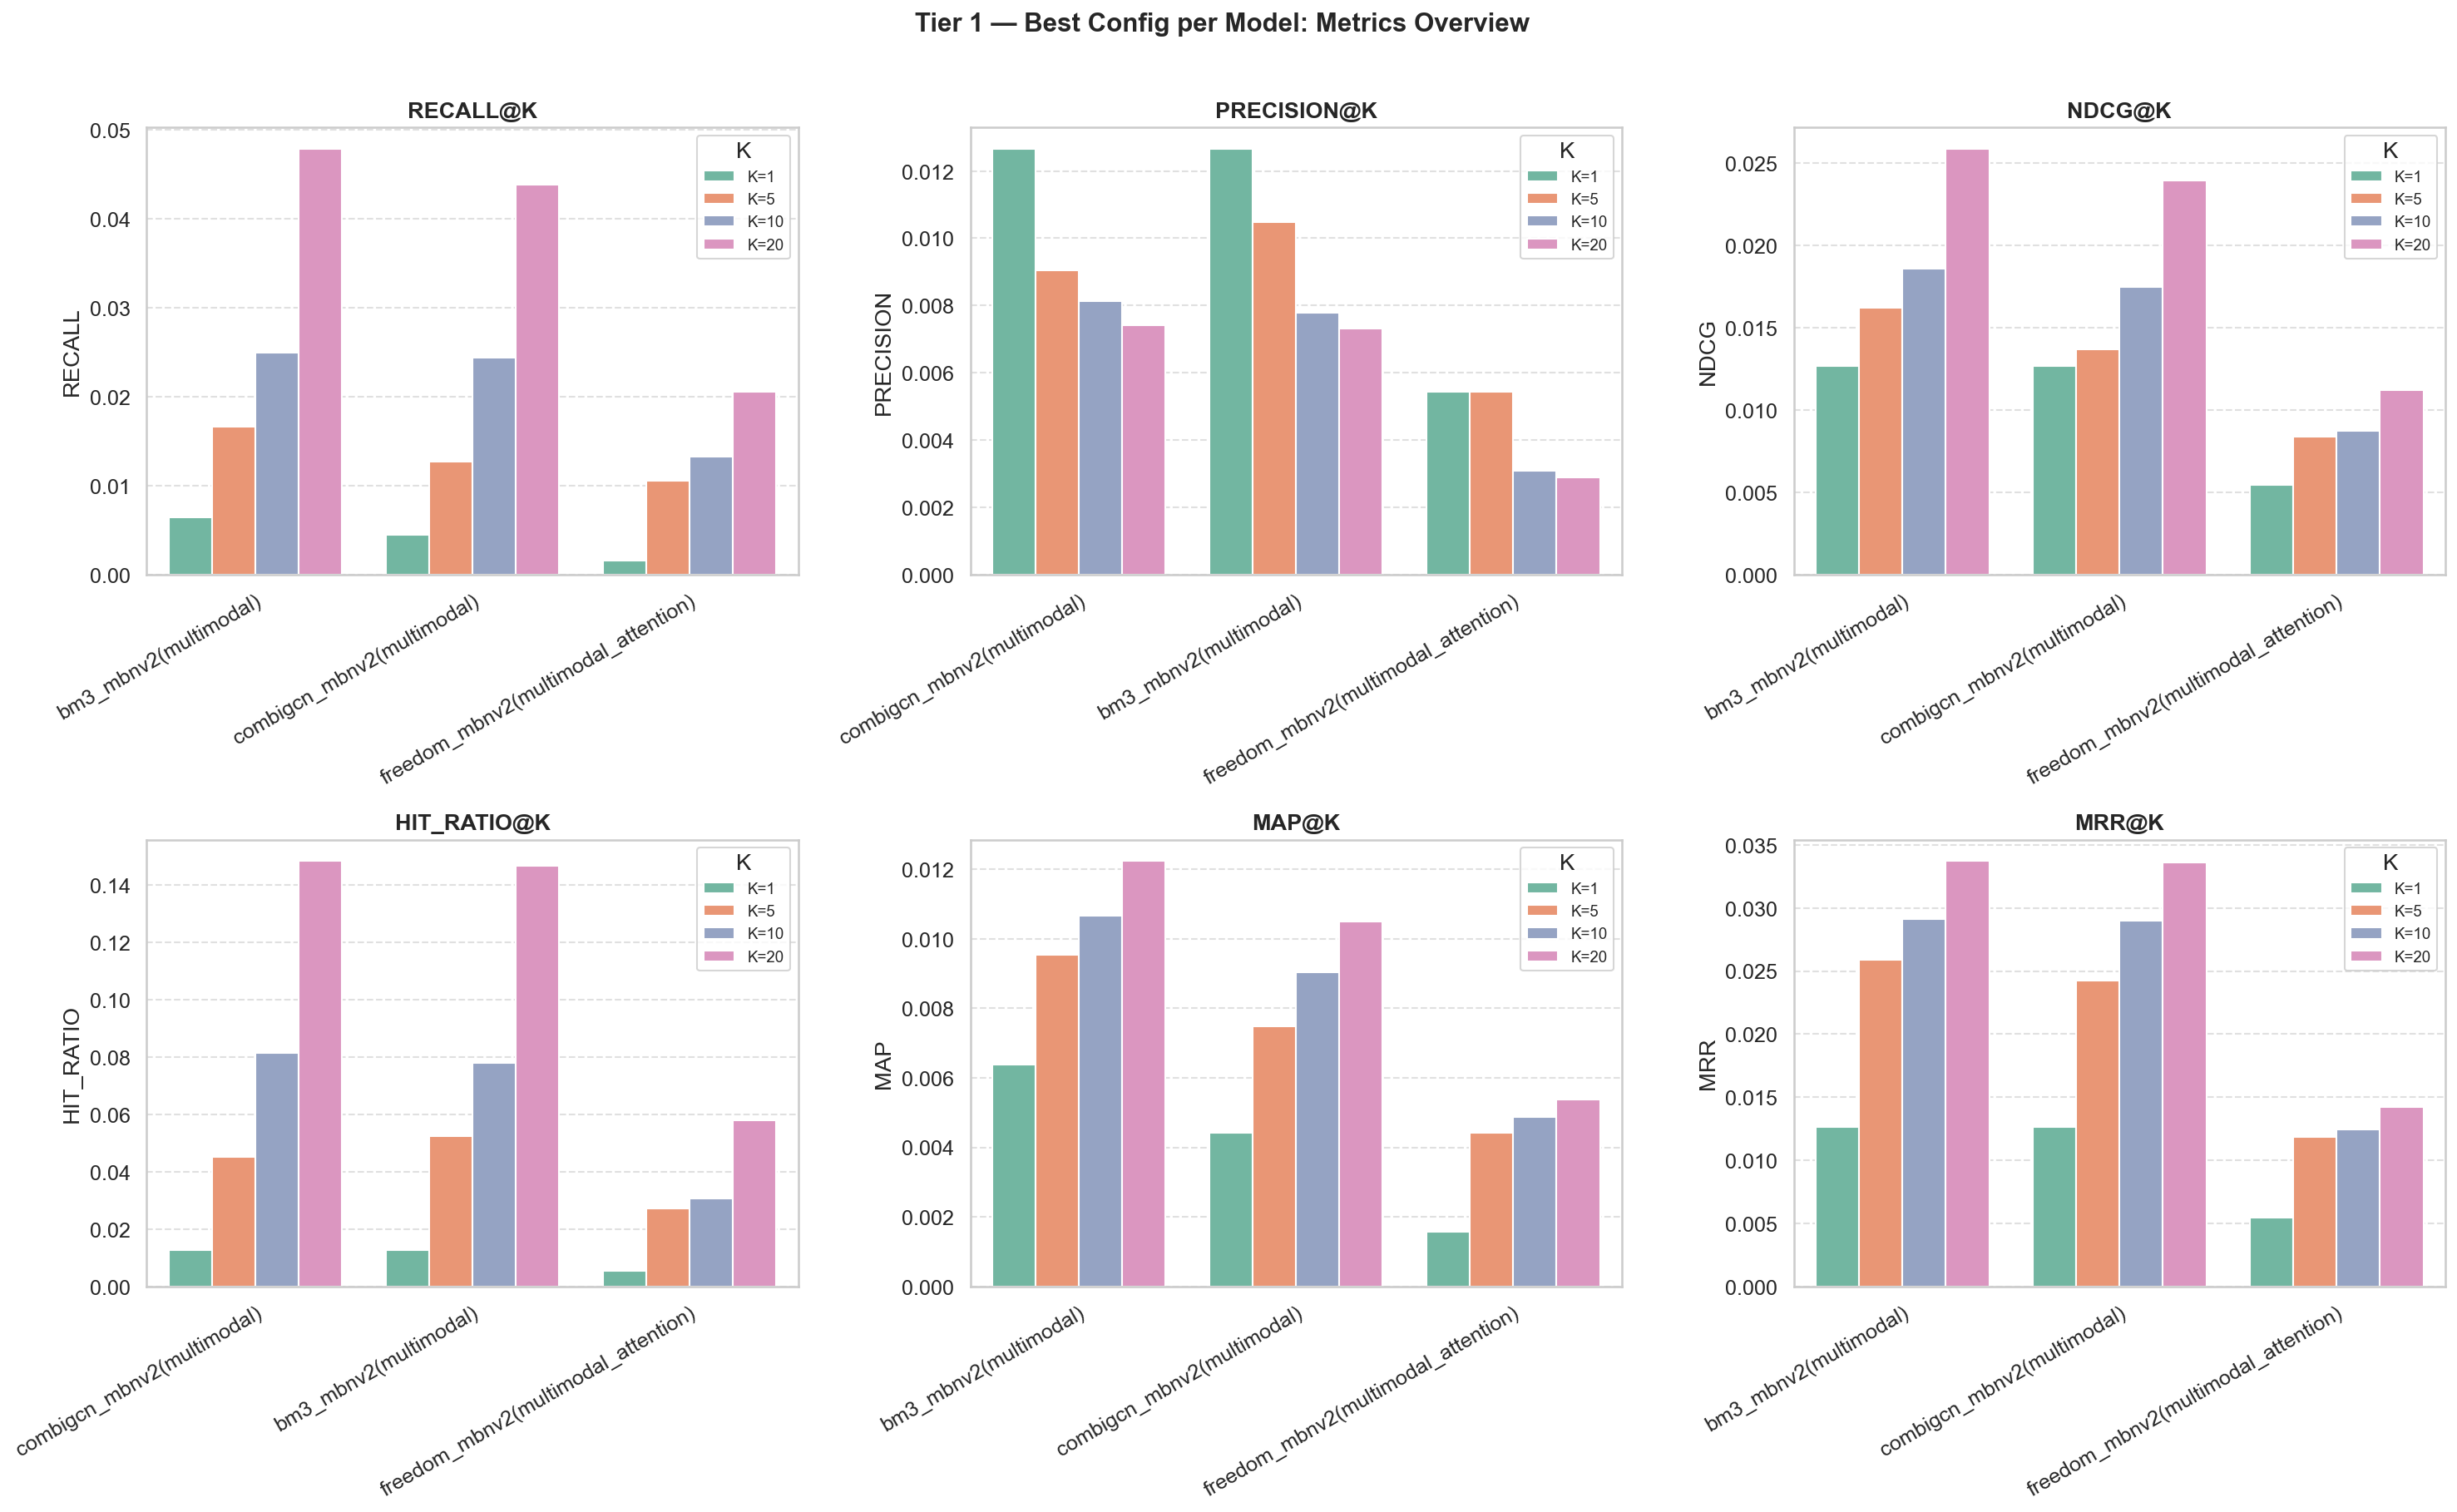
\includegraphics[width=0.8\textwidth]{figs/chap4/Figure_72_Tier_1_Best_Config_per_Model_Metrics_Overview.png}
    \caption{Comparison of the best configurations of BM3, CombiGCN, and FREEDOM across all six evaluation metrics.}
    \label{fig:best_config_overview}
\end{figure}

Detailed analysis of Figure~\ref{fig:best_config_overview} reveals the following performance trade-offs:
\begin{itemize}
    \item \textbf{BM3 vs. CombiGCN Performance Gap}: The performance gap between BM3 and CombiGCN is highly dependent on the ranking size $K$. At $K=10$, the performance gap is narrow, with BM3 leading by only $+6.3\%$ (NDCG of $0.0186$ versus $0.0175$). However, at $K=5$, the gap widens to $+18.4\%$ in favor of BM3 (NDCG of $0.0162$ versus $0.0137$). This demonstrates that BM3 possesses a significantly stronger ranking capability at top positions. Evaluating at $K=5$ is crucial because the test set contains only $3.81$ items per user on average; at $K=10$, recall saturation obscures these structural advantages.
    \item \textbf{Inverse performance at $K=1$}: We observe an important exception at $K=1$, where CombiGCN outperforms BM3 in both NDCG@1 and Precision@1. This implies that if a recommendation interface has a strict single-item constraint (demanding a precise first suggestion), CombiGCN is the superior choice. However, BM3 dominates from $K \ge 5$.
    \item \textbf{Underperformance of FREEDOM}: FREEDOM's best configuration is highly uncompetitive, achieving an NDCG@10 of only $0.0088$, which is $53\%$ lower than BM3. This shows that constructing an item-item kNN graph from raw visual/textual features introduces too much noise in sparse, small-scale datasets, unlike CombiGCN's stable precomputed similarity graph or BM3's contrastive bootstrap alignment.
\end{itemize}

\subsubsection{Consistency and Metric Coverage}

To verify the consistency of the findings and rule out metric bias, we analyze the mean performance across all values of $K \in \{1, 5, 10, 20\}$ in Figure~\ref{fig:best_overall_per_metric}.

\begin{figure}[H]
    \centering
    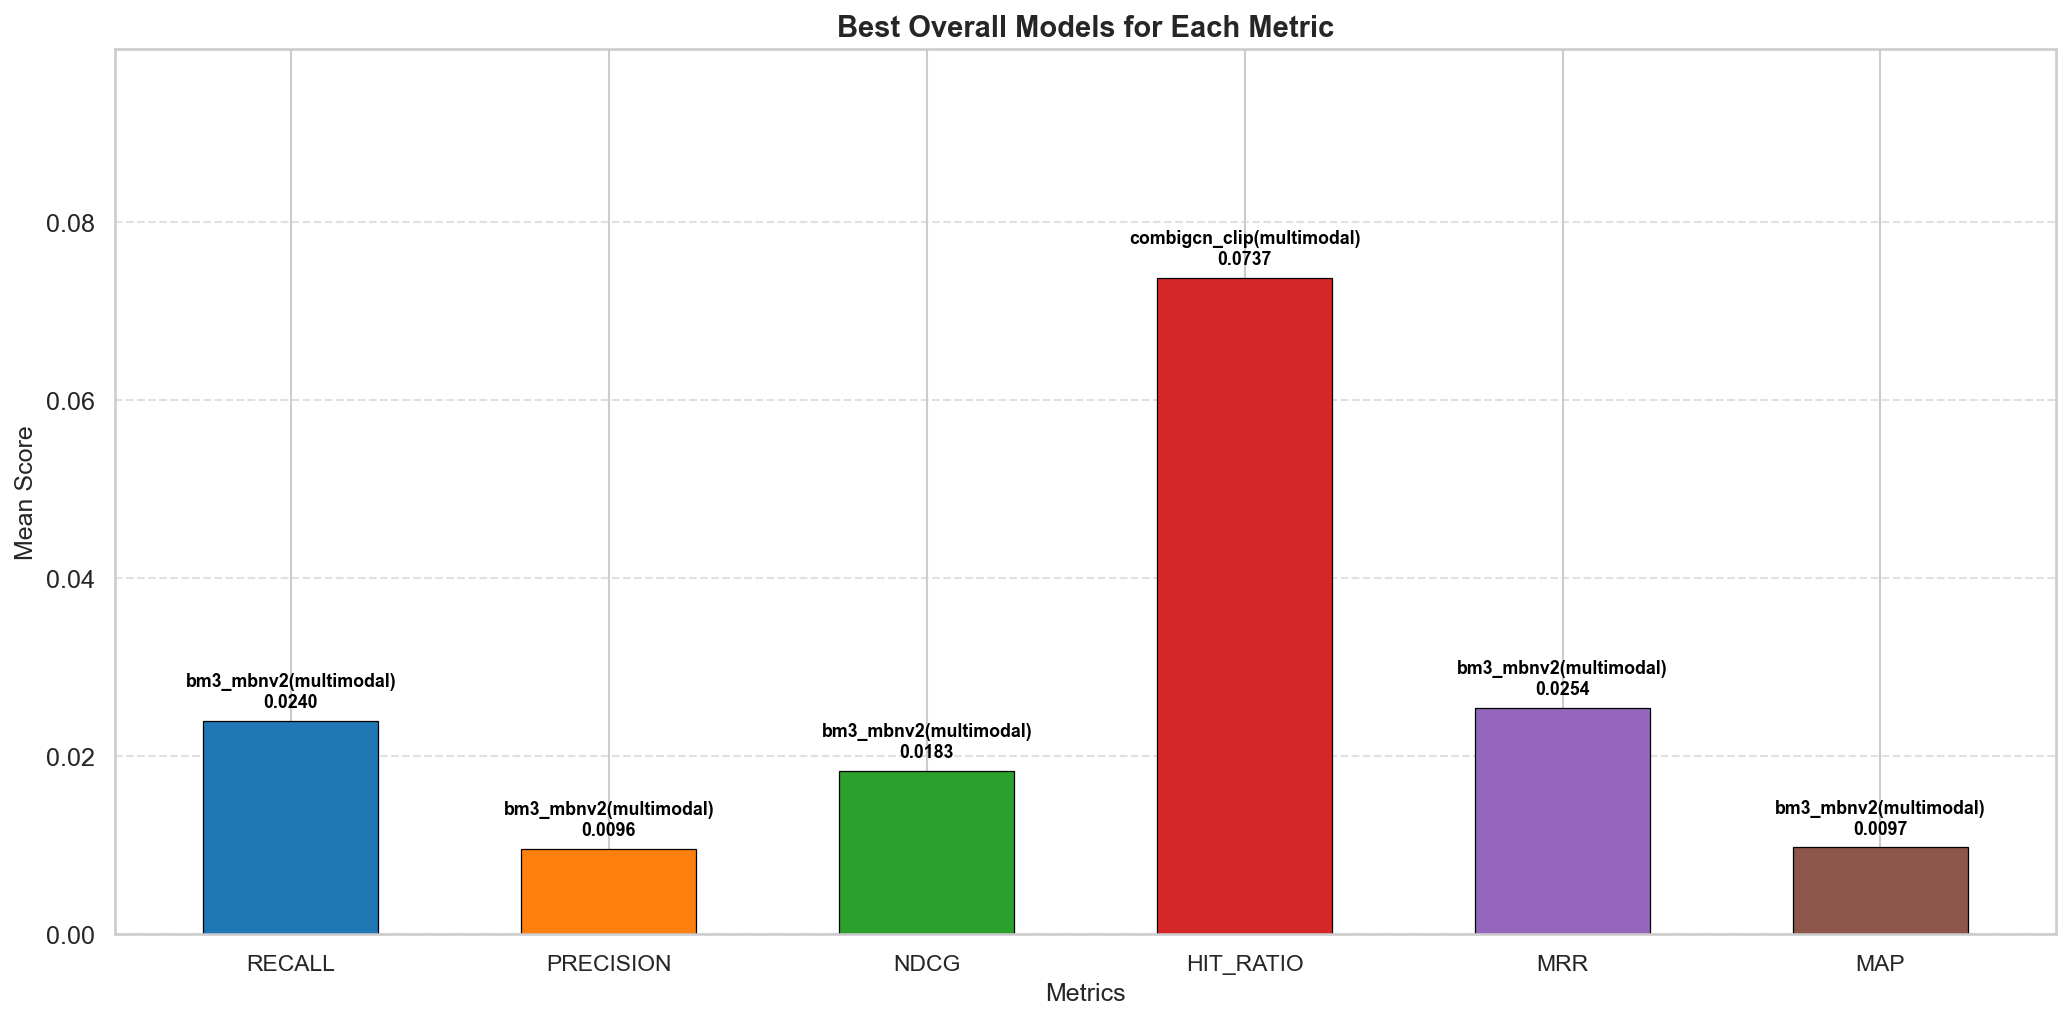
\includegraphics[width=0.7\textwidth]{figs/chap4/Figure_82_Best_Overall_Models_for_Each_Metric.png}
    \caption{Best overall performing model configuration for each recommendation metric, averaged across all $K$ cut-off values.}
    \label{fig:best_overall_per_metric}
\end{figure}

As shown in Figure~\ref{fig:best_overall_per_metric}, the optimal configuration of BM3 (\texttt{bm3\_mbnv2\_multimodal}) wins the highest average score in \textbf{5 out of 6 evaluation metrics}: Recall ($0.0240$), Precision ($0.0096$), NDCG ($0.0183$), MAP ($0.0097$), and MRR ($0.0254$). This global superiority confirms that BM3's performance advantage is robust and not an artifact of a single metric or retrieval depth.

We observe a notable anomaly in the Hit Ratio metric: the CLIP-based CombiGCN configuration (\texttt{combigcn\_clip\_multimodal}) wins the highest mean Hit Ratio of $0.0737$. This indicates that CombiGCN + CLIP is highly sensitive to placing at least one correct recommendation in the top list, though its actual ranking quality (as measured by NDCG, MRR, and MAP) remains inferior to BM3.

In summary, the performance hierarchy \texttt{BM3 > CombiGCN > FREEDOM} remains consistent across all ranking depths and metrics. The combination of MobileNetV2 visual embeddings with the multimodal late fusion strategy on the BM3 architecture represents the state-of-the-art configuration for this fashion recommendation benchmark.
